\begin{frame}
\frametitle{Definition of Scaling}
\begin{itemize}
	
	\item Ability to handle service loads
	
	\item Addition of resources
	
	
	\item Meeting demands of distributed systems
	
\end{itemize}
\end{frame}


\begin{frame}
\frametitle{Why do we need MANO Scaling?}

\begin{itemize}
	\item System Load
	\item Lifecycle management and service provisioning
	
\end{itemize}   
\end{frame}

\begin{frame}
\frametitle{Heterogeneity as an effect of Scaling}
\begin{itemize}
	\item Administration in MANO
	\begin{itemize}
		\item Infrastructure domain - based on type of resources like networking,compute, and storage environments.
		
		\item Tenant domain - based on type of the network services.
	\end{itemize}
	\item Multi-MANO interworking
	\begin{itemize}
		\item Two service platforms cooperate.
		\item One orchestrator interface on the other orchestrator.
	\end{itemize}
	
	
\end{itemize}
\end{frame}



\begin{frame}
\begin{figure}
	\centering
	\includegraphics[width=1\linewidth]{"images/ETSI approaches"}
	\caption{ETSI Approaches for Multiple Administrative domains \cite{de2018network}}
	\label{fig:etsi-approaches}
\end{figure}

\end{frame}

\begin{frame}
\frametitle{Scalability Techniques}

\begin{itemize}
	
	
	\item Service replication
	\begin{itemize}
		\item Clone services on other nodes.
		\item Additional resources are provided to handle larger service loads.
		
	\end{itemize}
	\item Service migration
	\begin{itemize}
		\item Placing service on a different node.
		\item Migrated service performs same role as the unstable node.
	\end{itemize}
	
\end{itemize}
\end{frame}

\begin{frame}
\begin{itemize}
	\item Service system scaling
	\begin{itemize}
		\item Monitoring the status of all nodes in a distributed system.
		\item Dynamic scaling.
		\item Global Scalability Management (GSM) - current status of the nodes.
		\item Regional Scalability Management (RSM) - installed on all service nodes.
	\end{itemize}
	
\end{itemize}
\end{frame}

\begin{frame}
\frametitle{Scalability Approaches}

\begin{itemize}
	
	\item Proactive Scaling - scheduled scaling
	\item Reactive Scaling - auto scaling
	\item Predictive Scaling - predicts traffic based on machine learning models.
	\item Heirarchical service placement - split into Execution Zones(EZ).
\end{itemize}   
\end{frame}

\begin{frame}
\frametitle{Types of Orchestration}

\begin{itemize}
\item Peer-to-Peer orchestration
\item Hierarchical orchestration
\end{itemize}

\end{frame}

\begin{frame}
\frametitle{SCrAMbLE depicting hierarchical orchestration}
\begin{figure}
	\centering
	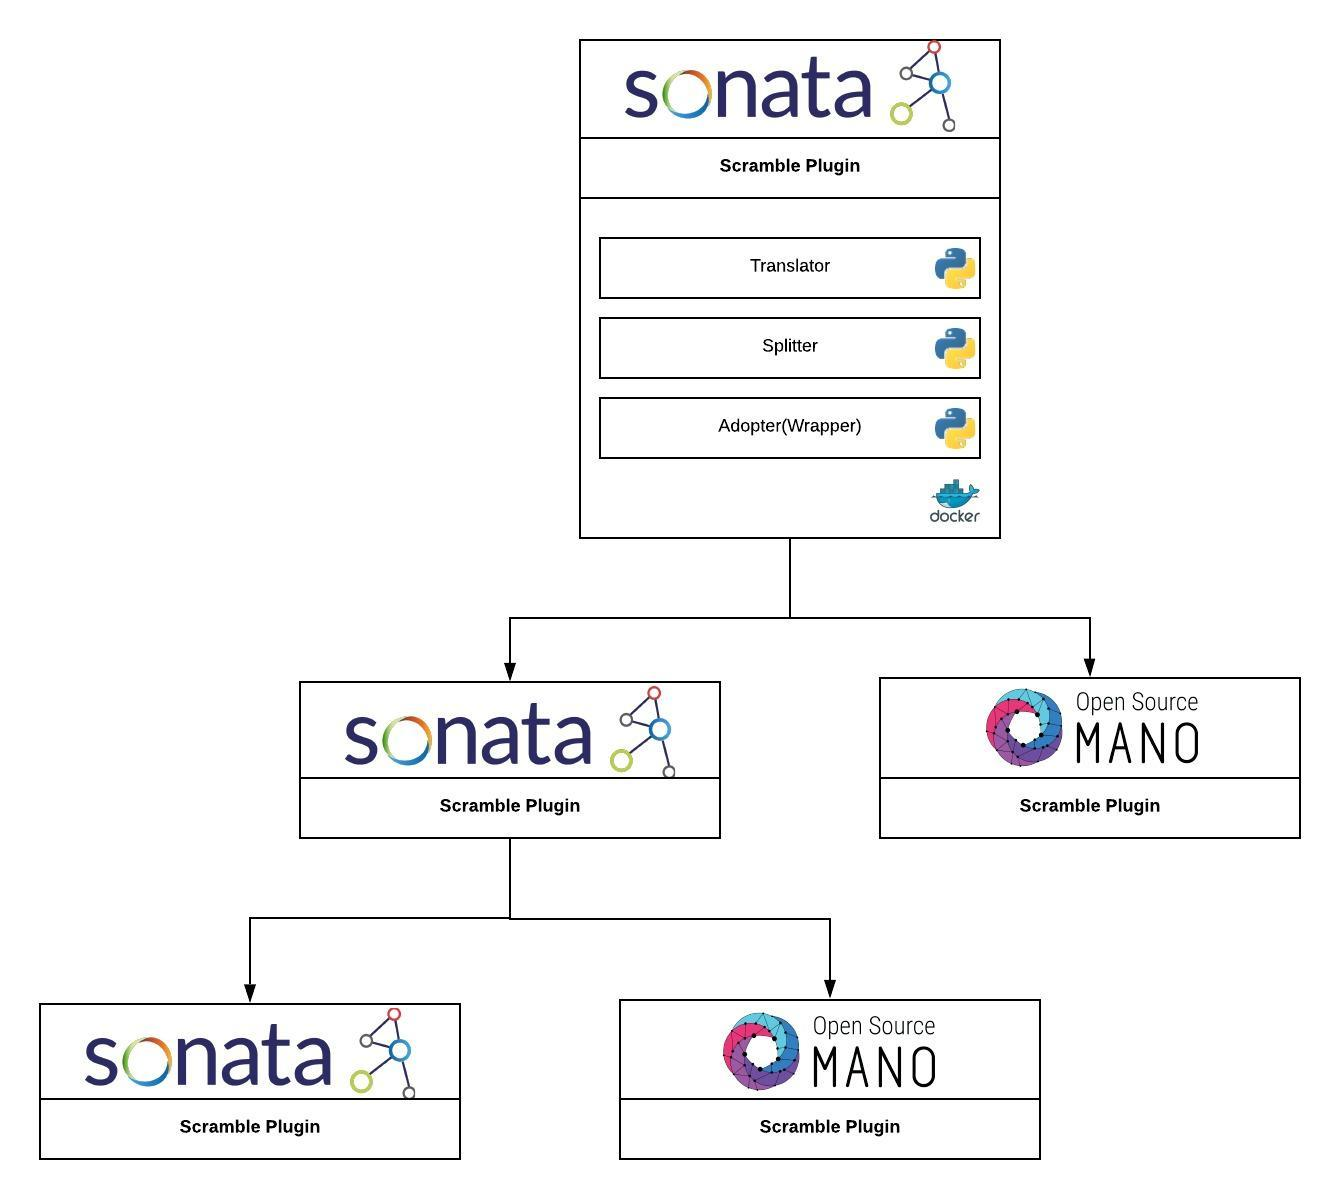
\includegraphics[width=0.7\linewidth]{images/scramblearch}
	\caption{High-level SCrAMbLE Architecture }
	\label{fig:scramblearch}
\end{figure}

\end{frame}

\begin{frame}
\frametitle{Hierarchical Orchestration}
\begin{itemize}
 

\item Using Hierarchical service placement technique.
\
\begin{itemize}
	\item Split  of EZs based on Resolution Domains(RDs).
	\item Higher level orchestrator makes the placement decision.
\end{itemize}
\item Minimum number of levels and number of MANOs required can be determined.
\end{itemize}
\end{frame}

\begin{frame}
\frametitle{References}
\begin{itemize}
	\item Nathan F Saraiva de Sousa, Danny A Lachos Perez, Raphael V Rosa, Mateus AS
	Santos, and Christian Esteve Rothenberg. Network service orchestration: A sur-
	vey. arXiv preprint arXiv:1803.06596, 2018. ii, 10
	
	\item Raul Muñoz, Ricard Vilalta, Ramon Casellas, Ricardo Martínez, Felipe Vicens,
	Josep Martrat, Víctor López, and Diego López. Hierarchical and recursive nfv
	service platform for end-to-end network service orchestration across multiple nfvi
	domains. In 2018 20th International Conference on Transparent Optical Networks
	(ICTON), pages 1–5. IEEE, 2018. 7
    
\end{itemize}
\end{frame}

